%
% einleitung.tex -- Beispiel-File für die Einleitung
%
% (c) 2020 Prof Dr Andreas Müller, Hochschule Rapperswil
%
% !TEX root = ../../buch.tex
% !TEX encoding = UTF-8
%
\section{Linienelemente\label{geodaeten:section:Linienelemente}}
\rhead{Linienelemente}

Ein Linienelement beschreibt, wie sich der Raum in die entsprechende Dimension verändert.
Es entspricht also der Ableitung einer Richtung nach der Zeit oder in anderen Worten um ein infinitesimales Wegelement.
In einem n-Dimensionalen Raum entspricht ein Linienelement also einem n-Dimensionalen Vektor, welcher die Änderung der Kurve in jeder Dimension beschreibt.
Um den Weg unsere Geodätenlinie minimieren zu können, müssen wir erst mal den Weg berechnen.
Jeder Weg kann in kleinere Wegstücke unterteilt werden, welche addiert wieder den ganzen Weg ergeben.
Da die Linienelemente den infinitesimalen Wegelementen entsprechen, müssen sie entlang jeder Dimension integriert werden.
Der Weg 'l' entspricht also der Summe von Wegstücken also
\begin{equation}
	l = \sum \Delta Weg
\end{equation}
und für infinitesimal große Wegstücke kann man diese ersetzen durch Linienelemente 'ds'  als
\begin{equation}	
	dWeg = ds .
	\label{geodaeten:Linienelemente:equation1}
\end{equation}
Um den Weg 'l' zu erhalten müssen schließlich diese Linienelemente in allen Dimensionen integrieren mit,
\begin{equation}
	l = 
	\sum^{n} \int_a^b ds .
	\label{geodaeten:Linienelemente:equation2}
\end{equation}

\section{Beispiele zu Linienelementen}
Die Beispiele sind für alle Unterkapitel gleich aufgebaut.
Zuerst wird das zweidimensionales Beispiel des Kartesischen Raumes als einfacher Einstieg behandelt.
Danach wird der Zylinder als einstieg in den dreidimensionalen Raum aufgezeigt.
Zum Schluss wird das Beispiel an einer Kugel untersucht, welches in der Praxis große Anwendung erfährt, aufgrund der Similarität zur Erdkugel.

	%
% einleitung.tex -- Beispiel-File für die Einleitung
%
% (c) 2020 Prof Dr Andreas Müller, Hochschule Rapperswil
%
% !TEX root = ../../buch.tex
% !TEX encoding = UTF-8
%
\subsection{Kartesisch\label{geodaeten:section:LinKartesisch}}
\rhead{Linienelemente Beispiele}

Wie in Abbildung [\ref{geodaeten:Linienelemente:figure1}] zu sehen ist kann ein Wegstück auf einer Kurve im zweidimensionalen Kartesischen Raum mit

\begin{equation}
	\Delta s \approx \sqrt{\Delta x^2 + \Delta y^2}
\end{equation}
approximiert werden.
Durch Verkleinerung der Wegstücke bis zum Infinitesimal 

\begin{equation}
	d s = \sqrt{d x^2 + d y^2}
	= \sqrt{\left(\frac{d x}{d t}\right)^2 \cdot d t^2 + \left(\frac{d y}{d t}\right)^2 \cdot d t^2} ,
\end{equation}
Kann das Linienelement aufgestellt werden als

\begin{equation}
 	ds^2 = \left(\dot{x}^2 +\dot{y}^2\right) \cdot dt^2 .
\end{equation}
Als Vektor dargestellt entspricht das Linienelement

\begin{equation}
	\mathbf{d\vec{s}}^2 = \begin{pmatrix} \dot{x}^2 \\ \dot{y}^2 \end{pmatrix} = \begin{pmatrix} 1 \\ 1 \end{pmatrix} \cdot \begin{pmatrix} \dot{x}^2 \\ \dot{y}^2 \end{pmatrix} \cdot dt^2 .
\end{equation}

\begin{figure}
	\centering
	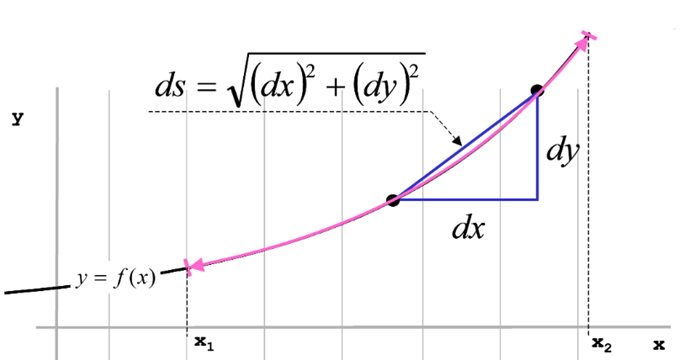
\includegraphics[width=0.7\linewidth]{papers/geodaeten/Abbildungen/Linienelemente/LinKartes1}
	\caption{Linienelement im Kartesischen Raum}
	\label{geodaeten:Linienelemente:figure1}
	\cite{geodaeten:kartesisch}
\end{figure}

	%
% einleitung.tex -- Beispiel-File für die Einleitung
%
% (c) 2020 Prof Dr Andreas Müller, Hochschule Rapperswil
%
% !TEX root = ../../buch.tex
% !TEX encoding = UTF-8
%
\subsection{Zylinder\label{geodaeten:section:Linienelemente:Zylinder}}
\rhead{Linienelemente Beispiele}

Eine Kurve auf der Oberfläche eines Zylinders kann als zweidimensional betrachtet werden, wobei gilt
\begin{equation}
	\Delta s \approx \sqrt{(r \cdot \Delta \phi)^2 + \Delta z^2}
\end{equation}
wenn $r$ konstant ist.
Analog zu den kartesischen Koordinaten können die Abstände infinitesimal werden und das Linienelement ergibt sich dadurch für die Oberfläche des Zylinders zu
\begin{equation}
	ds^2 = r^2 \cdot d \phi^2 + d z^2 .
	\label{geodaeten:equation:Linienelemente:Zylinder:equation2}
\end{equation}

Den Einstieg in dreidimensionale Kurven können wir machen, indem $r$ als nicht konstant angenommen wird.
Der Weg kann so mit
\begin{equation}
	\Delta s \approx \sqrt{\Delta r^2 + (r \cdot \Delta \phi)^2 + \Delta z^2} %\cdot dt^2
\end{equation}
berechnet werden und das Linienelement entspricht 
\begin{equation}
	ds^2 = d r^2 + r^2 \cdot d \phi^2 + d z^2 .
	\label{geodaeten:equation:Linienelemente:Zylinder:Zylinder3D}
\end{equation}

\begin{figure}
	\centering
	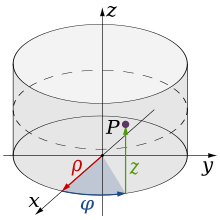
\includegraphics[width=4cm]{papers/geodaeten/Abbildungen/Linienelemente/LinZyl1}
	\caption{zylindrischer Raum mit $r = \rho$. Bildquelle: \cite{geodaeten:polarkoordinaten}}
	\label{geodaeten:figure:Linienelemente:Zylinder:figure2}
	
\end{figure}
	%
% einleitung.tex -- Beispiel-File für die Einleitung
%
% (c) 2020 Prof Dr Andreas Müller, Hochschule Rapperswil
%
% !TEX root = ../../buch.tex
% !TEX encoding = UTF-8
%
\subsection{Kugel\label{geodaeten:section:LinKugel}}
\rhead{Linienelemente Beispiele}

In ähnlicher Weise wie im Beispiel mit dem Zylinder lässt sich eine Kugel lokal wie eine flache Ebene darstellen.
Was auf den ersten Blick für sogenannte "Flat-Earther" ein schwieriges Konzept zu sein scheint, ist intuitiv verständlich:
Zoomt man nahe genug an die Erdoberfläche heran, verschwinden die Krümmungen, und Abstände lassen sich nahezu wie in einem euklidischen Raum berechnen.

In Kugelkoordinaten beschreibt $r$ den Abstand eines Punktes vom Zentrum der Kugel (Radius), $\theta$ den Winkel zur z-Achse (Polarwinkel), und $\phi$ den Winkel in der xy-Ebene (Azimutwinkel).
Diese Parameter definieren die Position eines Punktes auf der Kugeloberfläche eindeutig, wie in der Abbildung dargestellt.

Da wir uns auf der Oberfläche der Kugel befinden, bleibt $r$ konstant, und wir betrachten nur die Winkel $\theta$ und $\phi$.
Wenn ein Punkt nun um einen infinitesimalen Abstand auf der Kugeloberfläche verschoben wird, entstehen Verschiebungen entlang der zugehörigen Basisvektoren:
$r \, d\theta$ für die Breitenrichtung und $r \sin\theta \, d\phi$ für die Längsrichtung.

Weil lokal gerechnet werden kann wie in einem euklidischen Raum, ergibt sich der Abstand zwischen zwei Punkten auf der Kugeloberfläche durch die Anwendung des Pythagoras auf die jeweiligen infinetsimalen Verschiebungen entlang der Basisvektoren.

Das Linienelement $ds$ für die Oberfläche der Kugel kann daher als
\begin{equation}
ds^2 = r^2 \, d\theta^2 + r^2 \, \sin^2\theta \, d\phi^2
\end{equation}
beschrieben werden.

\begin{figure}
	\centering
	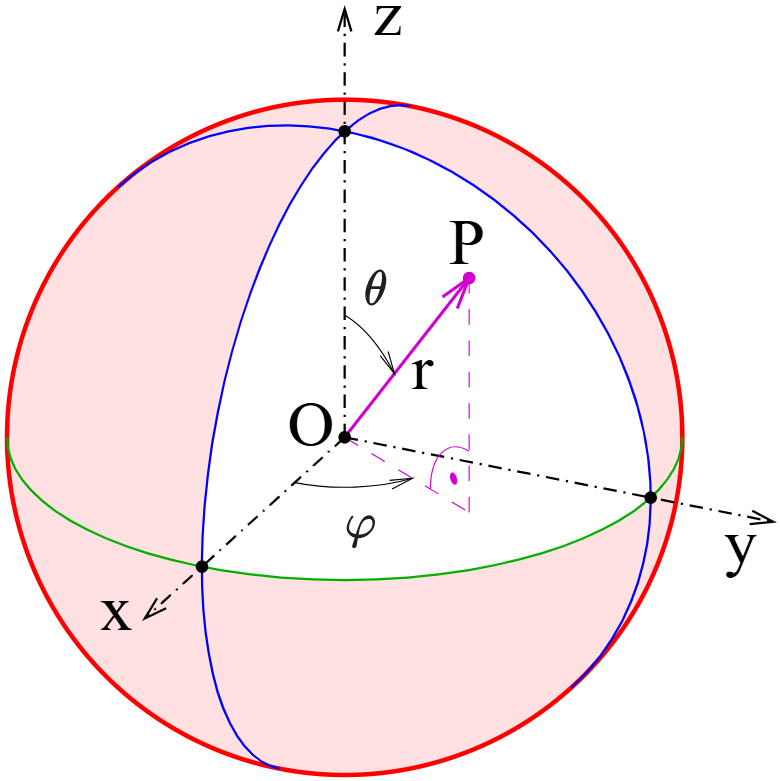
\includegraphics[width=0.7\linewidth]{papers/geodaeten/Abbildungen/Linienelemente/LinKugel1}
	\caption{Kugelkoordinaten mit Radius $r$, Polarwinkel $\theta$ und Azimutwinkel $\phi$}
	\label{geodaeten:figure:Linienelemente:Kugelkoordinaten}
	\cite{geodaeten:Kugelkoordinaten}
\end{figure}


